

\section{Dataset analysis}\label{sec:results:data}

This section contains an analysis of the available datasets. Some of the datasets are very large and later in the thesis all datasets were not used as the runtime was so long. For example not all datasets were handled in the parameter analysis in \sectionref{sec:parameters}. Specifically the datasets \textit{alpha}, \textit{alpha2} and \textit{eswc2015music} are often excluded and \textit{eswc2015movies} is also excluded sometimes.

The data is analyzed in two ways. Firstly the number of interactions is examined, both with respect to users and to items. All datasets are found to be top heavy, with \textit{alphaS} less so, with few very popular items encompassing most of the user base. Secondly clusters in the datasets is searched for with respect to compactness, or user similarities, using \textit{k-means} and on connectivity using \textit{spectral clustering}. Connected clusters are identified in all datasets.


\subsection{Number of interactions}\label{sec:result:interactions}

What follows is some graphs describing the number of interactions each user has and the number of interaction each item has in the datasets.

The graph on the left describe how many users have a fixed number of item interactions and conversely the graph on the right describe how many items have a set number of user interactions. The histograms are also represented in logarithmic scale.

\FloatBarrier

\twopic{fig/data/alphaS_items_per_user.png}{fig/data/alphaS_users_per_item.png}{
\textit{alphaS}
}

In \textit{alphaS} each user and each item has interactions with a small fraction of the available items and users. There are many users with very few interactions and also many items which few users has interacted with. There are no users or items without any interactions, but there are 11923 out of 16444 users and 2588 items out of 5000 with with only one interaction. This can be compared to the 26035 total interactions in the dataset. There are some users with more than 400 interactions and some items which have interacted with more 600 users.

\newpage

\twopic{fig/data/eswc2015books_items_per_user.png}{fig/data/eswc2015books_users_per_item.png}{
\textit{eswc2015books}
}

\twopic{fig/data/eswc2015movies_items_per_user.png}{fig/data/eswc2015movies_users_per_item.png}{
\textit{eswc2015movies}
}

\twopic{fig/data/eswc2015music_items_per_user.png}{fig/data/eswc2015music_users_per_item.png}{
\textit{eswc2015music}
}

\FloatBarrier

All \textit{eswc} datasets have similar distributions with more concentrated interactions. There is a lower limit for the number of interactions each user has, this is probably a constraint used when the datasets were made.
There are also no extreme user outliers with many more interactions than the norm.

The item interactions are more spread, with many items having interacted with relatively few user but some items having a lot of interactions. \textit{eswc2015books} have 1134 out of 2609 items with only one user interaction. \textit{eswc2015movies} and \textit{eswc2015music} in comparison have 2 out of 5389 items and 1 out of 6372 items with one user interaction.

\newpage

\twopic{fig/data/movielens1m_items_per_user.png}{fig/data/movielens1m_users_per_item.png}{
\textit{movielens1m}
}

\twopic{fig/data/romeo_items_per_user.png}{fig/data/romeo_users_per_item.png}{
\textit{romeo}
}

Both \textit{movielens1m} and \textit{romeo} have a more normalized look to them, especially with the number of user interactions per item compared to the other datasets. There are still outliers with many more interactions however. There are no users with less than 2 item interactions and there are no items without a user interaction. 114 out of 3706 items and 17 of 722 items have 1 user interaction in \textit{movielens1m} and \textit{romeo} respectively.

\FloatBarrier

In general two distinct types of users can be identified. The first is a user with only a couple of item interactions, this appears to be the most common type of user. It could possibly be users who try out a service but for some reason they do not continue or they are new users who just recently started using the service. The other user type is the one with a lot of item interactions, way more than the norm, and they are quite rare
\footnote{Parallels can be drawn to what is known as big spenders or ``whales'' in the social-gaming community. They make up a tiny group of the community but they drive most of the revenue for the game publishers. For a more in depth discussion see \\
VentureBeat: What it means to be a ``whale'' — and why social gamers are just gamers, 2013. \\
\url{http://venturebeat.com/2013/03/14/whales-and-why-social-gamers-are-just-gamers/} }
. They do not exist in the \textit{eswc} datasets.

A similar classification can be made for items. The vast majority of items has only a couple of user interactions. Perhaps these are new items few users have found out about or niche items not interesting to most users. 
A large fraction of the items in \textit{alphaS} and \textit{eswc2015books} have only one interaction (51\% and 43\%).  Then there are items with a lot more user interactions than what is common.

The following graphs display the number of the most popular items and the number of users they collectively interact with. This is useful for investigating how top heavy the datasets are. The dashed lines represents the number of items required to include 95\% of all users, a summary of the required number of items can be found in \tableref{tab:top_data}.

\begin{table}[h!]
    \centering
    \begin{tabular}{| c | r | r | r | r | r | l |}
        \hline
        \textbf{dataset}        & \textbf{items needed}  & \textbf{items total} & \textbf{item ratio}  \\ \hline

        \textit{alphaS}         &   3058          & 5000 & 61\%              \\ \hline
        \textit{eswc2015books}  &   120           & 2609 & 4.6\%                \\ \hline
        \textit{eswc2015movies} &   55            & 5389 & 1.0\%               \\ \hline
        \textit{eswc2015music}  &   78            & 6372 & 1.2\%               \\ \hline
        \textit{movielens1m}    &   13            & 3706 & 0.35\%               \\ \hline
        \textit{romeo}          &   21            & 722  & 2.9\%               \\ \hline

    \end{tabular}
    \caption{This table describes how many of the most used items are necessary to include in a set so 95\% of all users have interacted with the set.}
    \label{tab:top_data}
\end{table}

\twodiffpic{fig/data/alphaS_top_data.png}
{\textit{alphaS}. 3058 of 5000 (61\%) of the items are necessary to include 95\% of all users.}
{fig/data/eswc2015books_top_data.png}
{\textit{eswc2015books}. 120 of 2609 (4.6\%) of the items are necessary to include 95\% of all users.}

\twodiffpic{fig/data/eswc2015movies_top_data.png}
{\textit{eswc2015movies}. 55 of 5389 (1.0\%) of the items are necessary to include 95\% of all users.}
{fig/data/eswc2015music_top_data.png}
{\textit{eswc2015music}. 78 of 6372 (1.2\%) of the items are necessary to include 95\% of all users.}

\twodiffpic{fig/data/movielens1m_top_data.png}
{\textit{movielens1m}. 13 of 3706 (0.35\%) of the items are necessary to include 95\% of all users.}
{fig/data/romeo_top_data.png}
{\textit{romeo}. 21 of 722 (2.9\%) of the items are necessary to include 95\% of all users.}

%alphaS: 95\% of all users concentrated on 3058 of the items
%eswc2015books: 95\% of all users concentrated on 120 of the items (2609 tot, 4.6\%)
%eswc2015movies: 95\% of all users concentrated on 55 of the items (5389 tot, 1.02\%)
%eswc2015music: 95\% of all users concentrated on 78 of the items (6372 tot, 1.22\%)
%movielens1m: 95\% of all users concentrated on 13 of the items (3706 tot, 0.35\%)
%romeo: 95\% of all users concentrated on 21 of the items (722 tot, 2.91\%)

Of the different datasets, \textit{alphaS} is a clear outlier. It is nowhere near as top heavy as the other datasets are, requiring over 60\% of all items to reach 95\% of the users. This can in part be explained by the large number of users with only one interaction, 11923 out of 16444 users or in other words 72\% of all users have only one item interaction.
    
In contrast \textit{eswc2015books} require 4.6\% of the items and \textit{romeo} require 2.9\% of the items, which means few of the popular items are required to include most of the users. The other datasets are even more top heavy with \textit{eswc2015movies} and \textit{eswc2015music} only require 1.0\% and 1.2\% of the items. For \textit{movielens1m} only 0.35\%, namely 13, of the items are needed. In order words this means that 95\% of all users in the dataset has seen at least one movie from the 13 most watched movies.

This phenomena where very few of the most popular items command the attention of most of the user base is also seen in mobile app stores where 1.6\% of app developers make more than the other 98.4\% combined
\footnote{
readwrite: Among Mobile App Developers, The Middle Class Has Disappeared, 2014. \\
\url{http://readwrite.com/2014/07/22/app-developers-middle-class-opportunities}
}.

\FloatBarrier




\newpage
\subsection{Clusters}\label{sec:result:clusters}

Clustering with regards to compactness was examined using \textit{k-means} and with regards to connectivity using \textit{spectral clustering}. Compactness refer the closeness in space of the nodes in each cluster and connectivity refer to how connected the nodes in each cluster are with each other. In the recommendation domain compactness refers to how similar the users' full interaction history is to each other and connectivity instead examines similarity over user-item links.

As an example for two users who are close with respect to connectivity but not to compactness is when one user has a small subset of the other user's interactions.



\chapter{k-means clustering}\label{app:kmeans}

\textit{k-means clustering explanation here}
\Warning[TODO]{ Write! }


\newpage


\subsection{Connectivity using Spectral Clustering}

The process for clustering with spectral clustering is as follows
\footnote{A clear explanation of spectral clustering is given by \\
charlesmartin14: Spectral Clustering: A quick overview, 2012. \\
\url{https://charlesmartin14.wordpress.com/2012/10/09/spectral-clustering/}}

\begin{enumerate}
    \item Create an affinity matrix, or an adjacency matrix, $A_f$
    \item Construct a graph Laplacian $L$ from $A_f$
    \item Find eigenvalues and eigenvectors of $L$
    \item Select a subspace of eigenvectors
    \item Form clusters in the subspace
\end{enumerate}

In our particular case, the interaction matrix $A$ is defined as rows corresponding to users and columns corresponding to items. The affinity matrix needs to be square, but the interaction matrix is not. There are other more complex ways of creating an affinity matrix, but for this purpose modelling an adjacency matrix is sufficient.

A transformation from the interaction matrix $A$ to the adjacency matrix $A_{f}$ is made by having both users and items as both row and column indices and mirroring the interactions. $A_{f}$ will then be a symmetric, square matrix. Equation \eqref{eq:make_adj} illustrates an example of the matrix structure and \figureref{fig:spec:book:matrix} gives a concrete example for \textit{eswc2015books}.

As there are no connections between two users or between two items there will be two large zero rectangles in the top left and the bottom right.

\begin{equation}\label{eq:make_adj}
  A = \kbordermatrix{
    &    i_1 & i_2 & i_3 & i_4 \\
    u_1 & 0   & 1   & 0   & 1  \\
    u_2 & 0   & 1   & 1   & 1  \\
    u_3 & 1   & 0   & 1   & 0
  }
  \Rightarrow
    A_f = \kbordermatrix{
        &    u_1 & u_2 & u_3 & i_1 & i_2 & i_3 & i_4 \\
        u_1 & 0   & 0   & 0  &  0  &  1  &  0  &  1  \\
        u_2 & 0   & 0   & 0  &  0  &  1  &  1  &  1  \\
        u_3 & 0   & 0   & 0  &  1  &  0  &  1  &  0 \\
        i_1 & 0   & 0   & 1  &  0  &  0  &  0  &  0 \\
        i_2 & 1   & 1   & 0  &  0  &  0  &  0  &  0 \\
        i_3 & 0   & 1   & 1  &  0  &  0  &  0  &  0 \\
        i_4 & 1   & 1   & 0  &  0  &  0  &  0  &  0 \\
    }
\end{equation}

\begin{figure}[h!]
    \begin{subfigure}[h!]{0.5\textwidth}
        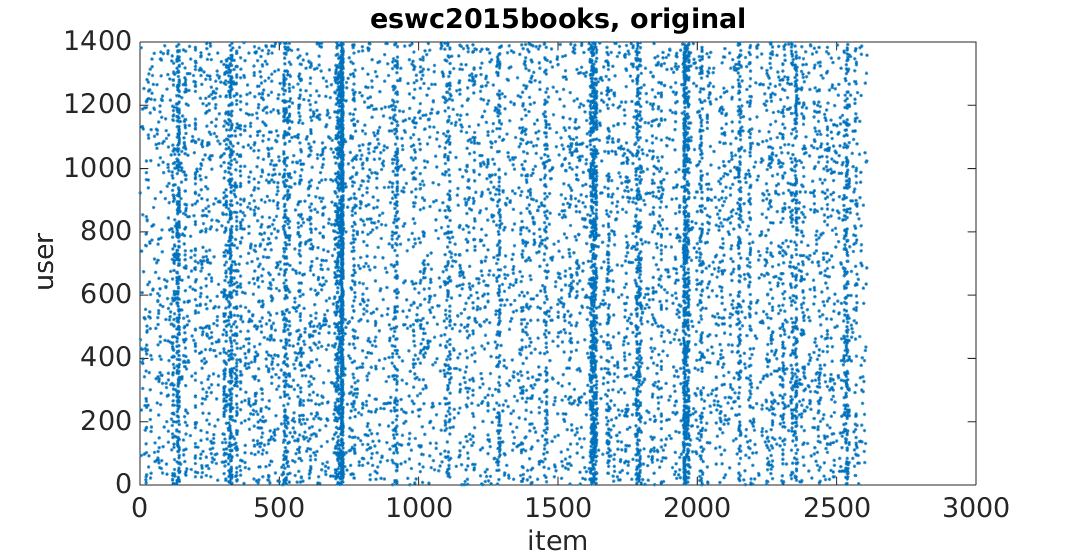
\includegraphics[width=\textwidth]{fig/spectral_data/eswc2015books_original.png}
        \caption{Interaction matrix $A$}
        \label{fig:spec:book:orig}
    \end{subfigure}
    ~
    \begin{subfigure}[h!]{0.5\textwidth}
        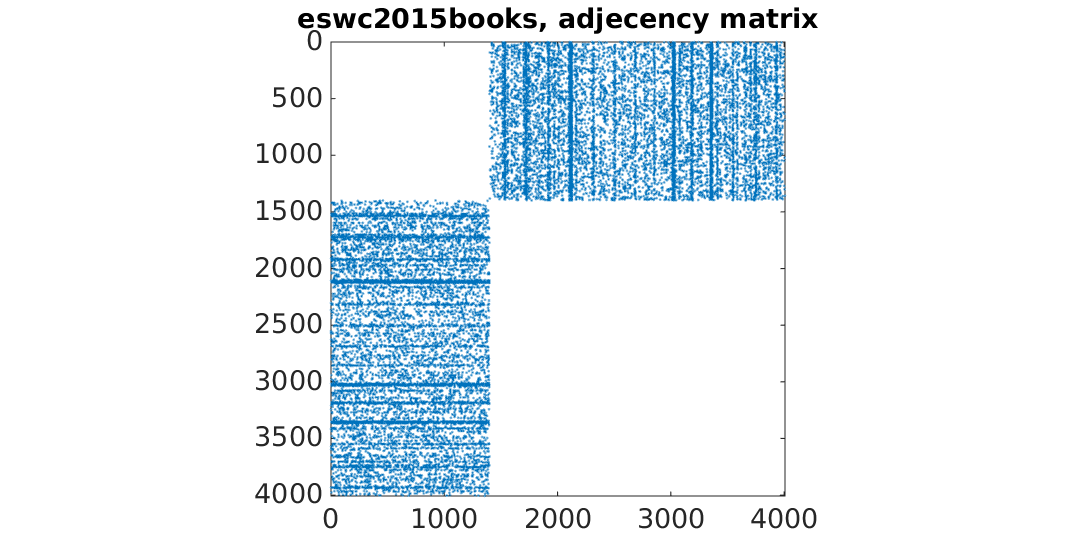
\includegraphics[width=\textwidth]{fig/spectral_data/eswc2015books_adj.png}
        \caption{Adjacency matrix $A_f$}
        \label{fig:spec:book:adj}
    \end{subfigure}
    \caption{This figure illustrates the original interaction matrix \ref{fig:spec:book:orig} for \textit{eswc2015books} and the related adjecency matrix \ref{fig:spec:book:adj}. Here the matrix $A$ has been moved to the upper right corner of $A_f$ as well as mirrored at the bottom left.}
    \label{fig:spec:book:matrix}
\end{figure}

There are different kinds of Laplacians, mostly differing in how the normalization is done. The one used here is the Generalized Laplacian $L$,

\begin{equation}
    L = D^{-1}( D - A_f )
\end{equation}

where $D$ is a diagonal matrix called the degree matrix. Each diagonal element $D_{i, i}$ represent the sum of degrees at each node $i$, calculated as the sum of row $i$,

\begin{equation}
    D_{i, i} = \sum_j A_{i, j}
\end{equation}

The principal idea is that if good clusters can be identified, then the Laplacian $L$ is approximately block diagonal, with each cluster defined by a block. That is if there are 3 clusters as in \eqref{eq:Lex},

\begin{equation}\label{eq:Lex}
    L =
    \begin{pmatrix}
        L_{1, 1} & L_{1, 2} & L_{1, 3} \\
        L_{2, 1} & L_{2, 2} & L_{2, 3} \\
        L_{3, 1} & L_{3, 2} & L_{3, 3}
    \end{pmatrix}
    \sim
    \begin{pmatrix}
        L_{1, 1} & 0         & 0        \\
        0        & L_{2, 2}  & 0        \\
        0        & 0         & L_{3, 3}
    \end{pmatrix}
\end{equation}

then also the lowest eigenvalues and their related eigenvectors correspond to different clusters. In this case the 3 smallest eigenvalues and eigenvector pair would correspond to each cluster, or block, in $L$.

To be able to identify different clusters, the sorted eigenvalues must have a gap. \Figureref{fig:spec:book:eigv} gives a concrete example for \textit{eswc2015books} (another example of clear clusters is \figureref{fig:spec:alphaS:eigv} for \textit{alphaS}). It is reasonable to expect there to be clear clusters in the adjacency matrix $A_f$, as there is a clear gap in the sorted eigenvalues. Note that this doesn't mean that there are clusters in the interaction matrix $A$, as there is duplicate information in $A_f$. There might be large areas without interactions, but the indexes might correspond to user-user or item-item which will not have any interactions. But it's a reasonable expectation.

The subspace to find clusters in is some subset of the eigenvectors corresponding to the smallest eigenvalues. The subspace used here is simply the eigenvector corresponding to the 2nd smallest eigenvalue \footnote{A practical example which used the same subspace is used as a reference. \\
Spectral Graph Partitioning and the Laplacian with Matlab, 2006. \\
\url{https://www.cs.purdue.edu/homes/dgleich/demos/matlab/spectral/spectral.html}
}.
\Figureref{fig:spec:book:eigsort} displays the adjacency matrix $A_f$ for \textit{eswc2015books} ordered by the ordering used when sorting the subspace. 

%There is some kind of structure in the graph, but it's hard to identify what it represents. The expectation is to find clusters represented by squares along the diagonal and there are some outlines of squares along the diagonal.

\FloatBarrier

\twodiffpiclabel{fig/spectral_data/eswc2015books_eigv.png}
{The smallest eigenvalues of $L$ for \textit{eswc2015books}.}
{fig:spec:book:eigv}
{fig/spectral_data/eswc2015books_eig_sort.png}
{Adjacency matrix $A$ of \textit{eswc2015books}, sorted by the ordering used when sorting the 2nd smallest eigenvector of $L$.}
{fig:spec:book:eigsort}

The interpretation of \figureref{fig:spec:book:eigv} is that one clear cluster is to be expected due to the gap between the first and second eigenvalue. Some other blurred clusters can be expected as the eigenvalues increase with a decreasing amount. If there are clear clusters the expectation is see square along the diagonal in \figureref{fig:spec:book:eigsort}. There are some horizontal and vertical lines which might be outlines of some triangles, but it's hard to see.

If instead of simply sorting the subspace, \textit{k-means} is used to find a clustering in the subspace, and that ordering is then used to reorder the adjacency matrix. \Figureref{fig:spec:book:kmeans} displays the adjacency matrix $A_f$ for \textit{eswc2015books}. 

\FloatBarrier

\twodiffpiclabel{fig/spectral_data/eswc2015books_kmeans_sort.png}
{Adjacency matrix $A_f$ of \textit{eswc2015books}, subspace clustered with \textit{k-means}.}
{fig:spec:book:kmeans}
{fig/spectral_data/eswc2015books_spectral_clust.png}
{Interaction matrix $A$ of \textit{eswc2015books}, reordered using \textit{k-means} clustering information.}
{fig:spec:book:clust}

\FloatBarrier

The reordered adjacency matrix in \figureref{fig:spec:book:kmeans} reveal several apparent clusters, but this doesn't directly mean that there are clusters in the dataset as we already know there are large areas without interactions in the adjacency matrix. But using the same ordering to reconstruct the adjacency matrix by reordering both users and items clusters are revealed for \textit{eswc2015books}, shown in \figureref{fig:spec:book:clust}.

In contrast with the compactness clustering which only clustered on a user level, this time there is clustering information for both users and items, this is a substantial benefit.

What follows is a similar analysis for the other datasets.

\FloatBarrier

\twodiffpiclabel{fig/spectral_data/alphaS_eigv.png}
{The smallest eigenvalues of $L$ for \textit{alphaS}.}
{fig:spec:alphaS:eigv}
{fig/spectral_data/alphaS_eig_sort.png}
{Adjacency matrix $A$ of \textit{alphaS}, sorted by the subspace ordering.}
{fig:spec:alphaS:eigsort}

The large number of zero eigenvalues in \figureref{fig:spec:alphaS:eigv} suggests that there are many clusters in \textit{alphaS}. This can also be seen in \figureref{fig:spec:alphaS:eigsort} where actual clear squares along the diagonal can be seen, as opposed to \figureref{fig:spec:book:eigsort} for \textit{eswc2015books}.

\twodiffpiclabel{fig/spectral_data/alphaS_kmeans_sort.png}
{Adjacency matrix $A_f$ of \textit{alphaS}, subspace clustered with \textit{k-means}.}
{fig:spec:alphaS:kmeans}
{fig/spectral_data/alphaS_spectral_clust.png}
{Interaction matrix $A$ of \textit{alphaS}, reordered using \textit{k-means} clustering information.}
{fig:spec:alphaS:clust}

\FloatBarrier

The final clustering for \textit{alphaS} in \figureref{fig:spec:alphaS:clust} reveal that \textit{alphaS} does have a large number of distinct clusters.  From the clustering made here it's possible to identify groups of users with specialized interests, with a subset of appealing items. This could possibly be used to identify personas
\footnote{
A persona is a description for a class of users or a description of a typical user.
This is a requested feature from Comordo's e-commerce clients and spectral clustering could form a base for creating or researching personas for a specific dataset. This process however is not automated and it's just a bi-product of this thesis and it's not pursued further.
}
in the dataset.

\newpage
The adjacency matrices for the following datasets are not plotted and only the eigenvalues and the final clustering of the interaction matrix $A$ is presented. They are sufficient to draw conclusions from.

\FloatBarrier

\twodiffpiclabel{fig/spectral_data/eswc2015movies_eigv.png}
{The smallest eigenvalues of $L$ for \textit{eswc2015movies}.}
{fig:spec:eswc2015movies:eigv}
{fig/spectral_data/eswc2015movies_spectral_clust.png}
{Interaction matrix $A$ of \textit{eswc2015movies}, reordered using \textit{k-means} clustering information.}
{fig:spec:eswc2015movies:clust}

\twodiffpiclabel{fig/spectral_data/eswc2015music_eigv.png}
{The smallest eigenvalues of $L$ for \textit{eswc2015music}.}
{fig:spec:eswc2015music:eigv}
{fig/spectral_data/eswc2015music_spectral_clust.png}
{Interaction matrix $A$ of \textit{eswc2015music}, reordered using \textit{k-means} clustering information.}
{fig:spec:eswc2015music:clust}

\twodiffpiclabel{fig/spectral_data/movielens1m_eigv.png}
{The smallest eigenvalues of $L$ for \textit{movielens1m}.}
{fig:spec:movielens1m:eigv}
{fig/spectral_data/movielens1m_spectral_clust.png}
{Interaction matrix $A$ of \textit{movielens1m}, reordered using \textit{k-means} clustering information.}
{fig:spec:movielens1m:clust}

\FloatBarrier

\twodiffpiclabel{fig/spectral_data/romeo_eigv.png}
{The smallest eigenvalues of $L$ for \textit{romeo}.}
{fig:spec:romeo:eigv}
{fig/spectral_data/romeo_spectral_clust.png}
{Interaction matrix $A$ of \textit{romeo}, reordered using \textit{k-means} clustering information.}
{fig:spec:romeo:clust}


\newpage

Clusters are visible in the final clustering of the interaction matrix $A$ for all dataset, but with less clear clustering than for \textit{alphaS}. It's supported by their respective eigenvalue plot, with all datasets have a prominent gap but only a single eigenvalue of zero. \Figureref{fig:spec:romeo:eigv} show that there are two other groups of eigenvalues with a gap between them suggesting there might be more prominent clusters in the dataset, which is supported by the clustering in \figureref{fig:spec:romeo:clust}.

The datasets \textit{eswc2015movies}, \textit{eswc2015music} and \textit{movielens1m} also have clusters but they are messier than that of \textit{romeo} or \textit{alphaS}. Part of the reason is the visualization technique where a sparse interaction matrix will produce a cleaner visualization.

This analysis searched for a fixed number of clusters $k = 10$, with \textit{alphaS} using $k = 15$. It is by no means the optimal number of clusters and there might be more clusters in the datasets and there might fewer but ``better fitting'' clusters. The point of this analysis is not to cluster the datasets in an optimal way, but to examine if the datasets have any clusters.

It's very hard to make recommendations for a dataset without any similarity between users, a random dataset for example, and the existence of clusters show that there is some structure in the dataset which could be used to make predictions. The intuition is that in a well clustered dataset users are tightly coupled with users of similar taste and reduces the noise of outlining interactions and a better approximation of the user's preferences can be made.


\newpage



